\section{Parameters identification}

\begin{frame}{Overview of the performed tests}

    In order to control the system, we had to \textbf{identify the parameters of the system}.
    To do so, many experiments have been conducted:

    \begin{enumerate}
        \item \textbf{Direct measurement};
        \item \textbf{Sensor characterization};
        \item \textbf{Control-to-voltage dependency};
        \item \textbf{Inductance characterization};
        \item \textbf{Force validation}.
    \end{enumerate}

\end{frame}



\begin{frame}{Direct measurement}

    Many of the parameters of the system can be directly measured using a scale, a caliper or a voltmeter.

    \begin{table}[H]

        \centering
        \begin{tabular}{|c|c|c|}
            \hline
            \textbf{Parameter} & \textbf{Value} & \textbf{Units} \\
            \hline
            $g$                & $9.81$         & $m/s^2$        \\
            $m$                & $0.06157$      & $kg$           \\
            $r$                & $0.06125/2$    & $m$            \\
            $h$                & $0.098$        & $m$            \\
            $R_{0}$            & $4.17$         & $\Omega$       \\
            \hline
        \end{tabular}

        \caption{Directly measured parameters and constants}
        \label{tab:directly_measured_parameters}

    \end{table}

\end{frame}



\begin{frame}{Sensor characterization}

    \only<1>{

        Voltage to position mapping.

        \begin{figure}[H]
            \centering
            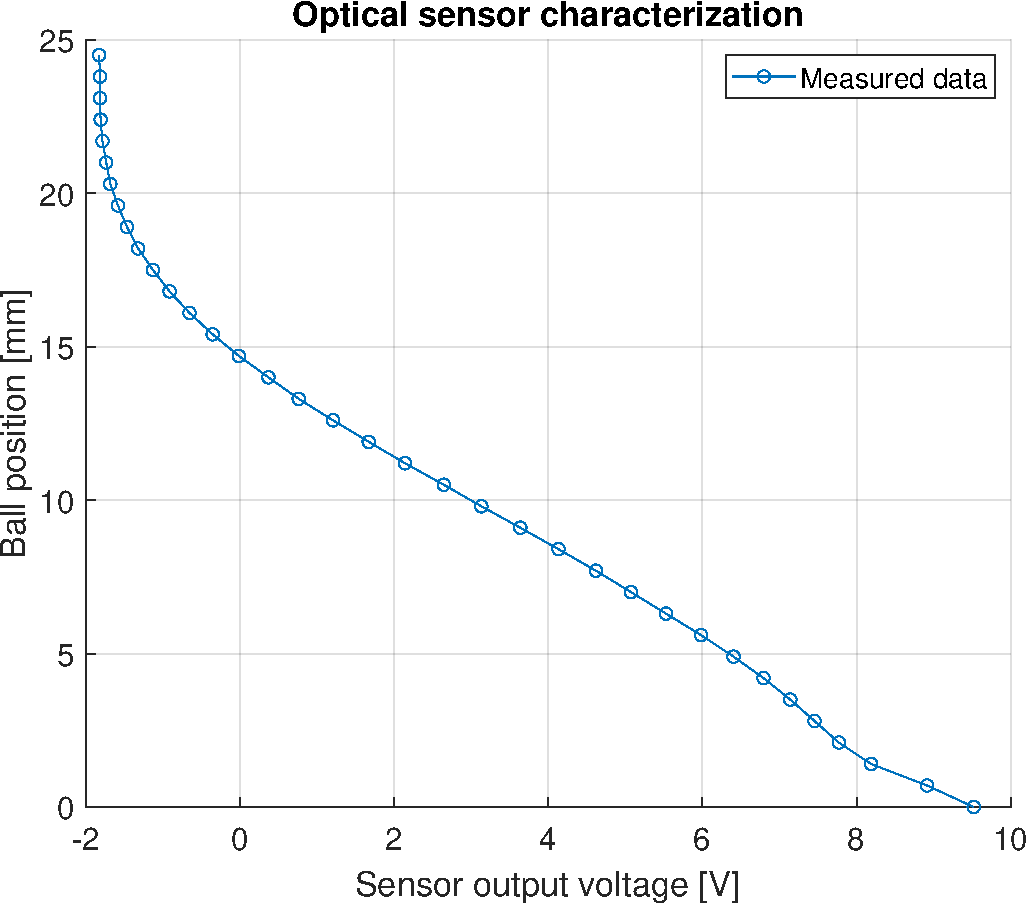
\includegraphics[width=0.6\textwidth]{img/MATLAB/identification/sensor_position.pdf}
            \caption{Position of the ball as a function of the output voltage of the infrared optical sensor.}
            \label{fig:voltage_to_position}
        \end{figure}

    }

    \only<2>{

        Sensors noise analysis.

        \begin{figure}[H]
            \centering
            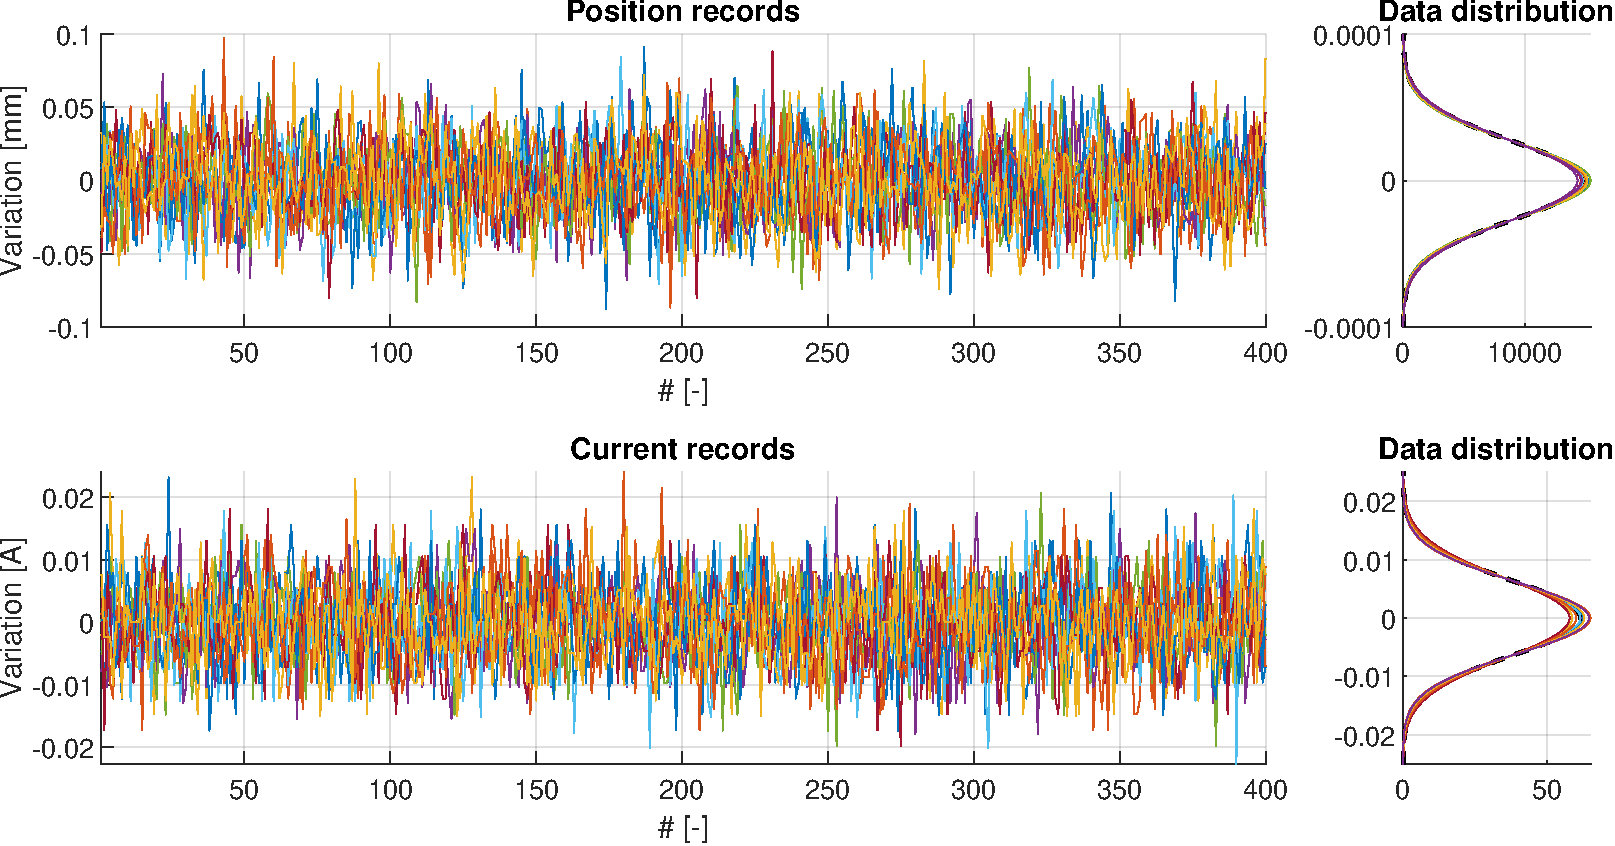
\includegraphics[width=1\textwidth]{img/MATLAB/identification/sensor_noises.pdf}
            \caption{Sensors' noise analysis.}
            \label{fig:sensors_noise}
        \end{figure}

        \begin{table}[H]
            \centering

            \begin{tabular}{|c|c|c|}
                \hline
                \textbf{Sensor} & \textbf{Standard deviation}        & \textbf{Covariance}                  \\
                \hline
                Infrared        & $1.402804 \cdot 10^{-3} \quad [m]$ & $7.166031 \cdot 10^{-6} \quad [m^2]$ \\
                Current         & $6.327979 \cdot 10^{-3} \quad [A]$ & $4.005490 \cdot 10^{-5} \quad [A^2]$ \\
                \hline
            \end{tabular}

            \caption{Standard deviation and covariance of the sensors' noise.}
            \label{tab:sensors_noise}

        \end{table}

    }


    \only<3>{
        Control to Voltage mapping.

        \begin{columns}[c, onlytextwidth]

            \begin{column}{0.45\textwidth}

                As predictable, the control to voltage mapping is a linear function outside the `no control zone'.

                \begin{equation}
                    V = \begin{cases}
                        V_{min} & \text{if } U < U_{min}    \\
                        k U + c & \text{if } U \geq U_{min}
                    \end{cases}
                \end{equation}

            \end{column}

            \begin{column}{0.55\textwidth}

                \begin{figure}
                    \centering
                    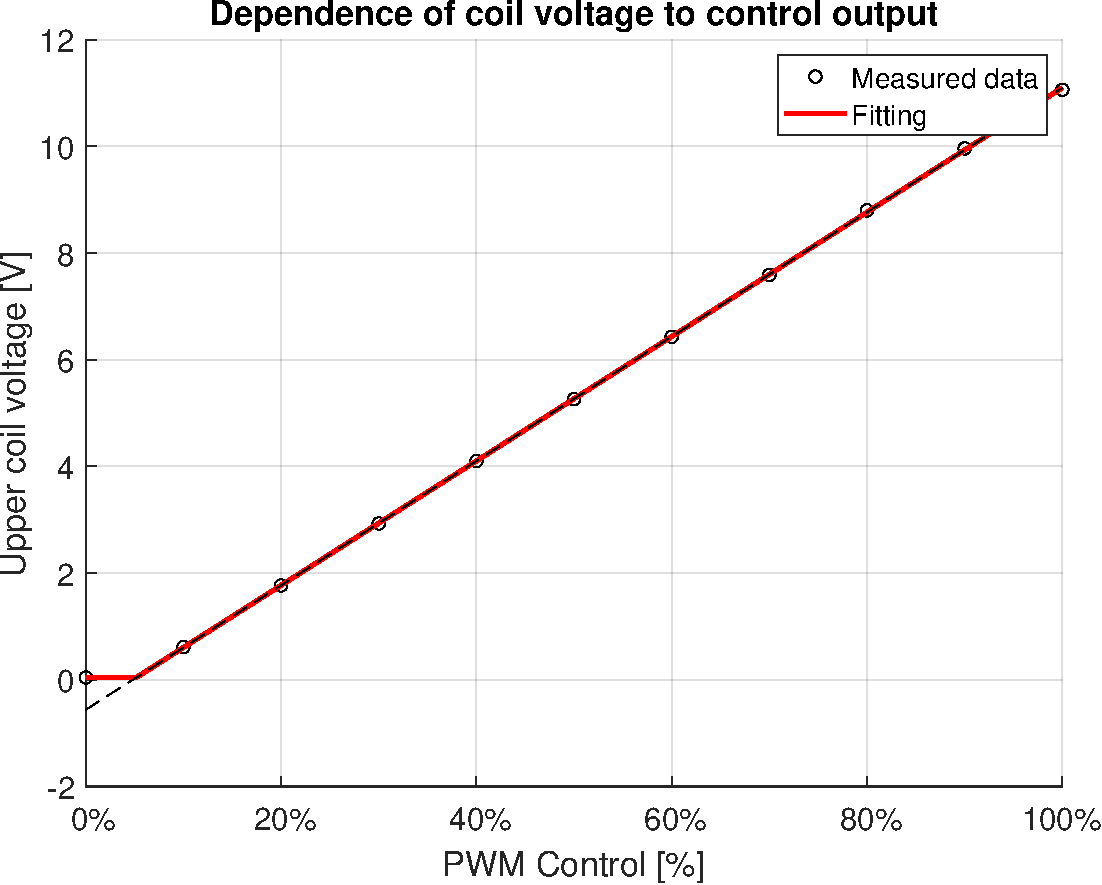
\includegraphics[width=0.8\textwidth]{img/MATLAB/measurements/control_to_voltage.pdf}
                    \caption{Voltage as a function of $U$}
                \end{figure}

            \end{column}

        \end{columns}

    }

    \only<3>{
        Electromagnetic force characterizations.

        \begin{columns}[c, onlytextwidth]

            \begin{column}{0.65\textwidth}

                \begin{figure}
                    \centering
                    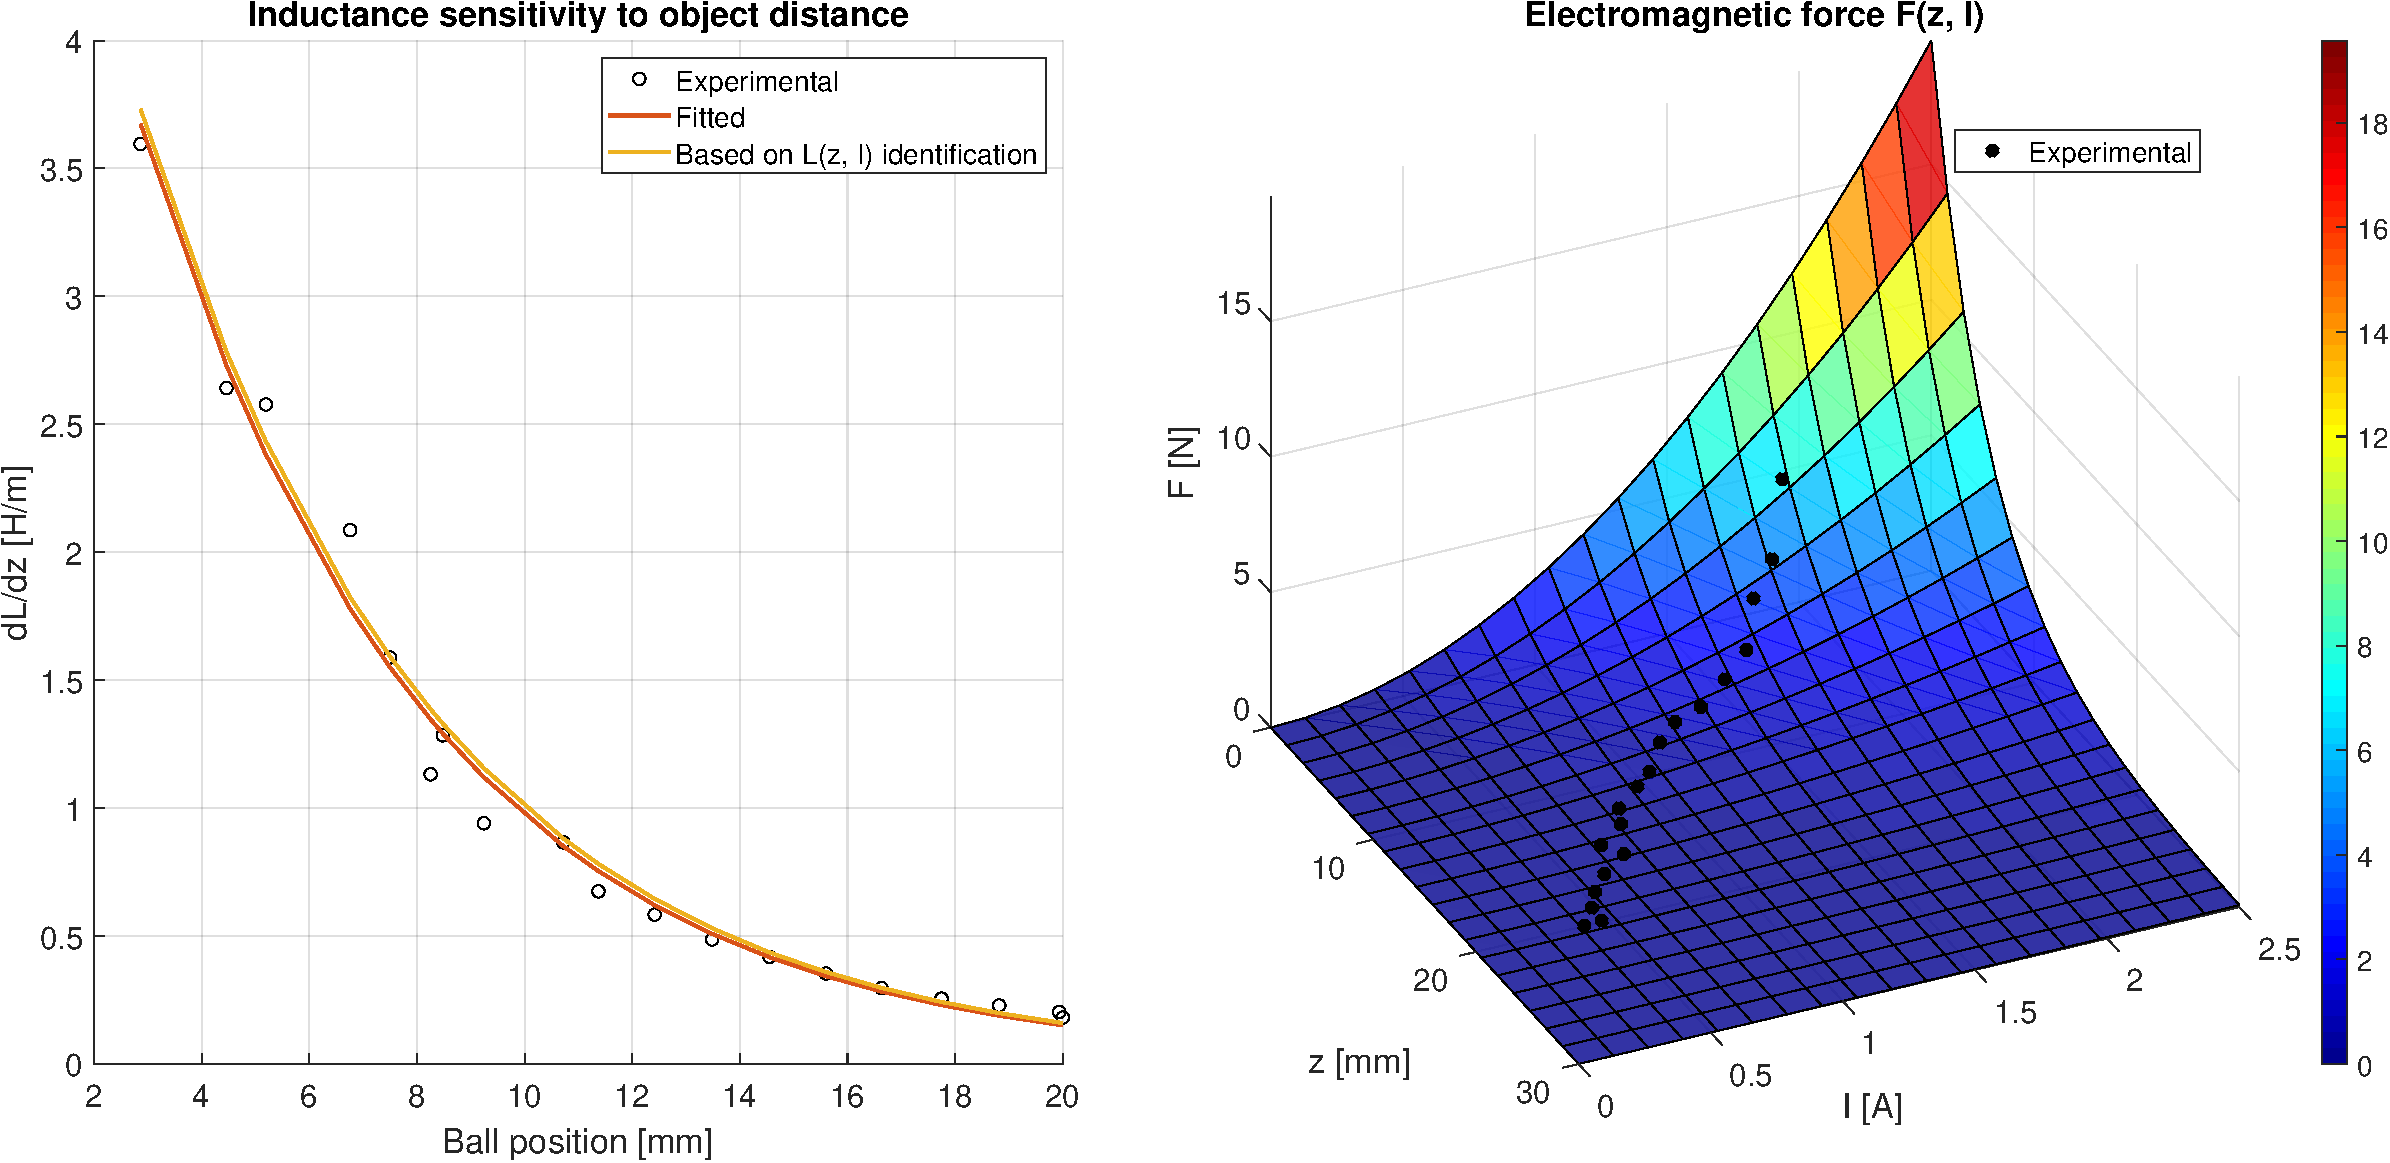
\includegraphics[width=0.8\textwidth]{img/MATLAB/measurements/force.pdf}
                    \caption{Electromagnetic force as a function of $z$ and $I$}
                \end{figure}

            \end{column}

            \begin{column}{0.35\textwidth}

                Notice that from the theoretical model, we have found the electromagnetic force acting on the ball to be:

                \begin{equation}
                    F_{em} = \frac{1}{2} \frac{\partial L}{\partial z} I^2
                \end{equation}

            \end{column}

        \end{columns}

    }

\end{frame}